\graphicspath{{conceptImages/}}
\chapter{Concept}

\section{Dialogue homme-machine}

Le dialogue est un discours que l’on construit à deux, s’il y a plusieurs personnes, on parle alors de multilogue.
\vspace{1em}

	Il y a un langage oral avec un niveau très variable ; il peut être spontané, avec la présence d’hésitations,  de corrections et de répétitions.
	\vspace{1em}
	
	Sa construction se fait avec des tours de paroles, avec la possibilité de parler plus fort que l’autre, de couper l’autre en plein milieu d’une phrase ou encore de l’empêcher de parler.
	\vspace{1em}
	
	Pour finir, il y a une importance sur les aspects paralinguistiques (accents, intonation et rythme) et extralinguistiques (gestes de la main, de la tête, du regard et de la posture) qui donnent des sens cachés dans une conversation.
\vspace{1em}

	Pour le dialogue avec une machine, on veut utiliser les mêmes caractéristiques du dialogue à la différence que celui-ci n’a d’intérêt que lorsqu’il est finalisé en exécutant une tâche, ce pourquoi il a été créé.
	\vspace{1em}
	
	Les enjeux du dialogue homme-machine est de reproduire le dialogue conventionnel. Pour ça, il doit réussir à gérer les tours de paroles en conservant des informations données par l’utilisateur pour les réutiliser au bon moment, et plus il y a de tours et plus c’est compliqué.
	\vspace{1em}
	
	Il doit comprendre le langage naturel dans toute sa complexité, ce qui comprend l’orthographe et la grammaire d’une langue, on reviendra sur ce point dans la partie natural language understanding. Dans un langage oral avec un aspect cognitif, il doit tenter de comprendre au maximum les aspects para et extralinguistiques.
	\vspace{1em}
	
	Il y a plusieurs définitions du dialogue ;  je reprends celles utilisées dans une thèse sur le dialogue homme-machine :
	\vspace{1em}
	
Définition 1 : Le dialogue est l'ensemble des échanges entre un utilisateur et une machine (ou un ensemble de logiciels). \cite{ref7}
\vspace{1em}

	Le terme échange regroupe ici toutes les interactions possibles avec l’utilisateur, par dialogue écrit sur ordinateur, vocal, visuel et bien d’autres. Cette définition est une définition générale qui intègre les définitions 2 et 3. 
\vspace{1em}

Définition 2 : Le dialogue est l'ensemble des interactions produites par un humain sur un ordinateur. \cite{ref7}
\vspace{1em}

	Une interaction est une action qui provoque une réaction perceptible. Elle regroupe des notions telles que les clics souris, la frappe de touches, les pressions sur un écran tactile, etc.  Cette définition est la plus courante en matière d'IHM.
\vspace{1em}

Définition 3 : Le dialogue est l'utilisation du langage naturel pour travailler sur un ordinateur. \cite{ref7}
\vspace{1em}

\section{Natural Language processing}

Nous allons maintenant voir comment comprendre le langage naturel de l’utilisateur par la machine. Pour cela, on a le natural language  processing qui est l’approche informatique pour analyser du texte en se basant sur des théories et des connaissances.
\vspace{1em}

Définition : Le natural language processing est la théorie des techniques informatiques pour analyser et représenter des textes naturels sur plusieurs niveaux d'analyse linguistique afin de réaliser le traitement du langage semblable à l'homme pour un ensemble de tâches ou d’applications.
\vspace{1em}


\subsection{But}

Le but du NLP : il doit accomplir le traitement du langage semblable à l'homme. Le choix du mot «  traitement » est très délibéré et ne devrait pas être remplacé par de » la compréhension ». Bien que le domaine du NLP ait été à l'origine mentionné comme le Language Natural Understanding (NLU) dans les premiers jours de l’intelligence artificielle, il est bien accepté aujourd'hui que le but n'a pas encore été accompli. 
\vspace{1em}

Un Système NLU complet devrait être capable de :
\vspace{1em}

\begin{itemize}
	\item Paraphraser un texte en entrée
	\item Traduire le texte dans une autre langue 
	\item Répondre aux questions en fonction du texte 
	\item Faire des déductions à partir du texte
\end{itemize}
\vspace{1em}

	Le but du système NLP est de représenter la vraie signification et l'intention de la question de l'utilisateur qui peut être exprimée naturellement dans le langage courant. Aussi, le contenu d’informations qui sont recherchées sera représenté à tous leurs niveaux de signification pour qu'un vrai matching entre le besoin et la réponse puisse être trouvé.


\subsection{Principes}

	Tandis que le domaine entier est mentionné comme le NLP, il y a en fait deux parties distinctes :  la compréhension du langage (NLU) et la génération de langue(NLG).
	\vspace{1em}
	
	Le premier de ceux-ci se réfère à l'analyse de la langue pour produire une représentation significative, tandis que le dernier se réfère à faire une production de la représentation. 
	\vspace{1em}
	
	Le NLP est équivalent au rôle de lecteur/auditeur, tandis que la tâche NLG est celle de l'auteur/orateur. Alors qu'une grande partie de la théorie et de la technologie est partagée par ces deux divisions, la Génération de Langage naturel exige aussi une capacité de planification. C'est-à-dire que le système de génération exige un modèle sur le but de l'interaction pour décider ce que le système doit produire à chaque interaction.
\vspace{1em}


\section{Natural language understanding}

	La méthode pour présenter ce qui arrive en réalité dans un système de traitement automatique des langues se fait grâce à l'approche du « niveau des langues ». Ceci est aussi mentionné comme le modèle synchrone de langue qui établit l’hypothèse suivante : les niveaux de traitement du langage humain se suivent d’une façon strictement séquentielle. La recherche psycholinguistique suggère que le traitement du langage soit beaucoup plus dynamique de même que les niveaux peuvent interagir dans une variété d'ordres. 
\vspace{1em}
		
Par exemple, la connaissance pragmatique que le document que vous lisez est de la sociologie sera utilisé quand un mot particulier qui a plusieurs sens est rencontré et le mot sera interprété comme ayant du sens pour la sociologie. 
	\vspace{1em}
	
La description des niveaux de langage sera présentée séquentiellement (figure \ref{fig:Cycle d'analyse d'une phrase})

	\vspace{1em}
	
\begin{figure}[H]
	\centering
		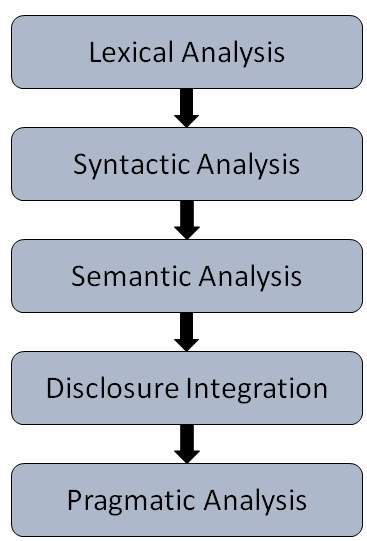
\includegraphics[width = 0.5\textwidth]{phaseAnalyse.png}
	\caption{Cycle d'analyse d'une phrase}
	\label{fig:Cycle d'analyse d'une phrase}
\end{figure}

Le point clé consiste ici en ce que la signification soit transmise par chaque niveau de langue et que l'on gagne en compréhension.
\vspace{1em}

	Ce processus implique trois problèmes majeurs : le premier se rapporte à la façon de penser, le deuxième à la représentation et à la signification linguistique et le troisième au domaine de connaissance.
	\vspace{1em}
	
	 Ainsi, un système NLP peut commencer au niveau d’un mot pour déterminer la structure morphologique, la nature … et peut ensuite avancer au niveau de la phrase pour déterminer l'ordre des mots, grammaire, signification de la phrase entière. Après, il y a le contexte et l'environnement global. Un mot donné ou une phrase peuvent avoir une signification spécifique ou une connotation dans un contexte donné et peuvent être liés à beaucoup d'autres mots et phrases dans le contexte donné.
	\vspace{1em}

\subsection{Phonologie}

	Ce niveau traite l'interprétation des sons vocaux à travers les mots. En fait, il y a trois types de règles utilisées dans l'analyse phonologique : 
	\vspace{1em}
	
	\begin{enumerate}
		\item règles phonétiques, pour les sons dans les mots
		\item des règles phonémiques, pour les variations de voix
		\item règles prosodiques, pour la fluctuation causée par le stress, les accents et l’intonation à travers une phrase
	\end{enumerate} 
\vspace{1em}

	Dans un système NLP qui accepte un dialogue vocal, les ondes sonores sont analysées et codées dans un signal numérisé pour l'interprétation par des règles diverses ou par la comparaison au modèle de langue particulier étant utilisé.

\subsection{Morphologie}

Ce niveau traite la nature componentielle de mots qui sont composés de morphèmes, les unités les plus petites de signification. C’est une décomposition du sens d'un mot en unités de sens élémentaires. Par exemple, le mot reconstruction peut être morphologiquement analysé dans trois morphèmes séparés : le préfixe re-, la racine construc- et le suffixe -tion. Les humains peuvent décomposer un mot inconnu dans ses morphèmes constitutifs pour comprendre sa signification. De même un système NLP peut reconnaître la signification transmise par chaque morphème pour gagner et représenter la signification.

\subsection{Lexical}

	L’analyse lexicale consiste à décomposer une chaîne de caractères en entités lexicales et ranger ces entités dans des catégories ;  on appelle ce processus la segmentation.
\vspace{1em}
	
Il existe deux modèles :
\vspace{1em}

\begin{itemize}
	\item Lexicaux qui est une liste de mots de la langue ; par conséquent,  les mots inconnus ne sont pas reconnus… 
	\item Statistiques qui est la probabilité des successions de mots.
\end{itemize}
\vspace{1em}

À ce niveau, les humains aussi bien que les systèmes NLP  interprètent la signification de mots individuels. De plus, au niveau lexical, ces mots qui ont plusieurs sens possibles peuvent être remplacés par une représentation sémantique. La nature de la représentation varie selon la théorie sémantique utilisée dans le système NLP. 
\vspace{1em}

	Le niveau lexical peut exiger un lexique et l'approche particulière prise par un système de NLP qui déterminera quel lexique sera utilisé. Les lexiques peuvent être tout à fait simples, avec seulement les mots, ou peuvent être de plus en plus complexes et contenir des informations sur la classe sémantique du mot. 

\subsection{Syntaxique}

	L’analyse syntaxique étudie la façon dont les mots se combinent pour former des phrases dans une langue donnée.
	\vspace{1em}
	
	Ce niveau d'analyse des mots permet de découvrir la structure grammaticale de la phrase. Ceci exige tant la grammaire qu'un analyseur syntaxique. L’analyse de ce niveau est une représentation de la phrase qui révèle les relations de dépendance structurelles entre les mots. Il y a diverses grammaires qui peuvent être utilisées et qui auront un impact sur le choix de l’analyseur syntaxique. La syntaxe transmet la signification dans la plupart des langues parce que l'ordre et la dépendance contribuent à la signification. 
	\vspace{1em}
	
Par exemple les deux phrases : « le chien a poursuivi le chat. » et « le chat a poursuivi le chien. » diffèrent seulement en termes de syntaxe, et pourtant elles transmettent des significations tout à fait différentes.


\subsection{Sémantique}

L’analyse sémantique établit la signification d’une phrase en utilisant le sens de chaque motpar des formes logiques et/ou des formalismes gérant des formes logiques.
\vspace{1em}

Il existe 3 modèles impliqués : 
\vspace{1em}

\begin{itemize}
	\item Modèles fondés sur les référents,Théorie des Représentations Mentales (Reboul $1998$) et son implémentation (Grisvard $2000$) ; Représentations Référentielles (Popescu-Belis $2000$) ; Domaines de Référence (Salmon-Alt $2001$, Landragin $2003$)
	\item Modèles logiques, DRT (Kamp et Reyle $1993$) ; UDRT (Reyle $1993$) ; SDRT (Asher $1993$) ; MDRT (Pineda et Garza $2000$)
	\item Modèles statistiques, comme pour l’analyse lexical, on a la probabilité de succession de mot pour trouver un sens.
\end{itemize}
\vspace{1em}


Ce niveau de traitement peut inclure la désambiguïsation sémantique de mots avec des sens multiples.
\vspace{1em}

Par exemple, le mot « vienne » peut prendre plusieurs sens différents dans des phrases comme « qu'il vienne par là » (verbe « venir ») et dans d'autres comme « aller à Vienne » (nom propre). 
\vspace{1em}

	Du point de vue sémantique, le même mot « vienne », peut correspondre à la ville de « Vienne » qui existe en Autriche et en France, ainsi qu'au département de la Vienne. Il y a une multitude de mots ambigus dans toutes les langues, ce qui peut créer des incompréhensions. 
	\vspace{1em}
	
	Mais dans la perspective de l’analyse sémantique, en situation de communication réelle, on saura faire la différence dans un contexte entre les mots « Vienne » et « vienne ». Outre le V majuscule, la logique grammaticale permet de comprendre que « vienne » est un verbe, tandis que « Vienne » est un nom.
	
\subsection{Discours}

Tandis que la syntaxe et la sémantique travaillent sur l’analyse d’une phrase, le niveau de discours dans le NLP se concentre sur l’interprétation de l’enchaînement de phrases, dont chacune peut être interprétée séparément. Le discours se focalise sur les propriétés du texte qui se transmettent entre des phrases pour former des connexions. Plusieurs types de traitements de discours peuvent arriver à ce niveau, deux des plus communs étant la résolution d'anaphore et la reconnaissance de structures de discours/texte. 
\vspace{1em}

	La résolution d'anaphore est le remplacement de mots comme des pronoms, avec l'entité appropriée à laquelle ils se réfèrent. Par exemple, « Ma soeur a adopté un chat. Il n'est pas très beau ».
	\vspace{1em}
	
	La reconnaissance de structures de discours/texte détermine les fonctions des phrases  dans le texte, comme par exemple  thèse, antithèse et synthèse .
	
\subsection{Pragmatique}

L’analyse pragmatique identifie et traite les actes de langage que l’on catégorise selon leur but : citer, informer, conclure, donner un exemple, décréter, déplorer, objecter, réfuter, concéder, conseiller, distinguer, émouvoir, exagérer, ironiser, minimiser, railler, rassurer et rectifier. Mais elle traite aussi le second degré : présuppositions, implicitations, sous-entendus, sens littéral et sens argumentatif.
	\vspace{1em}
	
	Ce niveau est concerné par l'utilisation de la langue en prenant en compte le contexte et aussi le contenu pour comprendre quel est le but et expliquer les significations non visibles dans le texte. Ceci exige beaucoup de connaissances, y compris la compréhension des intentions, des plans et des buts du dialogue.
\subsection{Cognitive}

C’est un élément récent dans le dialogue homme-machine où l’on souhaite analyser les émotions de l’utilisateur. Cette analyse se fait par vidéo en reconnaissant des patterns du visages ou reconnaissance dans une phrase avec un modèle.

\subsection{Base de connaissance}

Les réponses dans un dialogue peuvent être générées à partir d’une base de connaissances pour répondre à l’utilisateur.


\section{Natural language Generation}


Après la phase d’analyse du natural language understanding, on a le natural language generation. Elle se base sur les résultats des analyses linguistiques (détermination du contenu sémantique de l’énoncé, résolution des références aux objets, identification des actes de langage) pour faire des hypothèses sur les intentions de l’utilisateur. 
\vspace{1em}

	Ensuite, on a un raisonnement sur ces hypothèses et sur l’intérêt de l’énoncé. L’énoncé courant est mis en rapport avec les énoncés précédents, c’est-à-dire qu’il faut gérer l’historique du dialogue pour trouver les réponses et les réactions pertinentes. 
	\vspace{1em}
	
Il existe 3 modèles impliqués :
\vspace{1em} 
\begin{itemize}
	\item Modèle de l’utilisateur avec une liste de préférences linguistiques, pragmatiques et des connaissances supposées.
	\item Historique du dialogue ou modèle de représentation des contenus échangés, pile des énoncés précédents et de leurs interprétations.
	\item Modèle de raisonnement sur les contenus, déductions logiques (ou pas).
\end{itemize}

\vspace{1em}

Voici (figure \ref{fig:Analyse NLP}) une représenation des phases énoncées précédemment :

\begin{figure}[H]
	\centering
		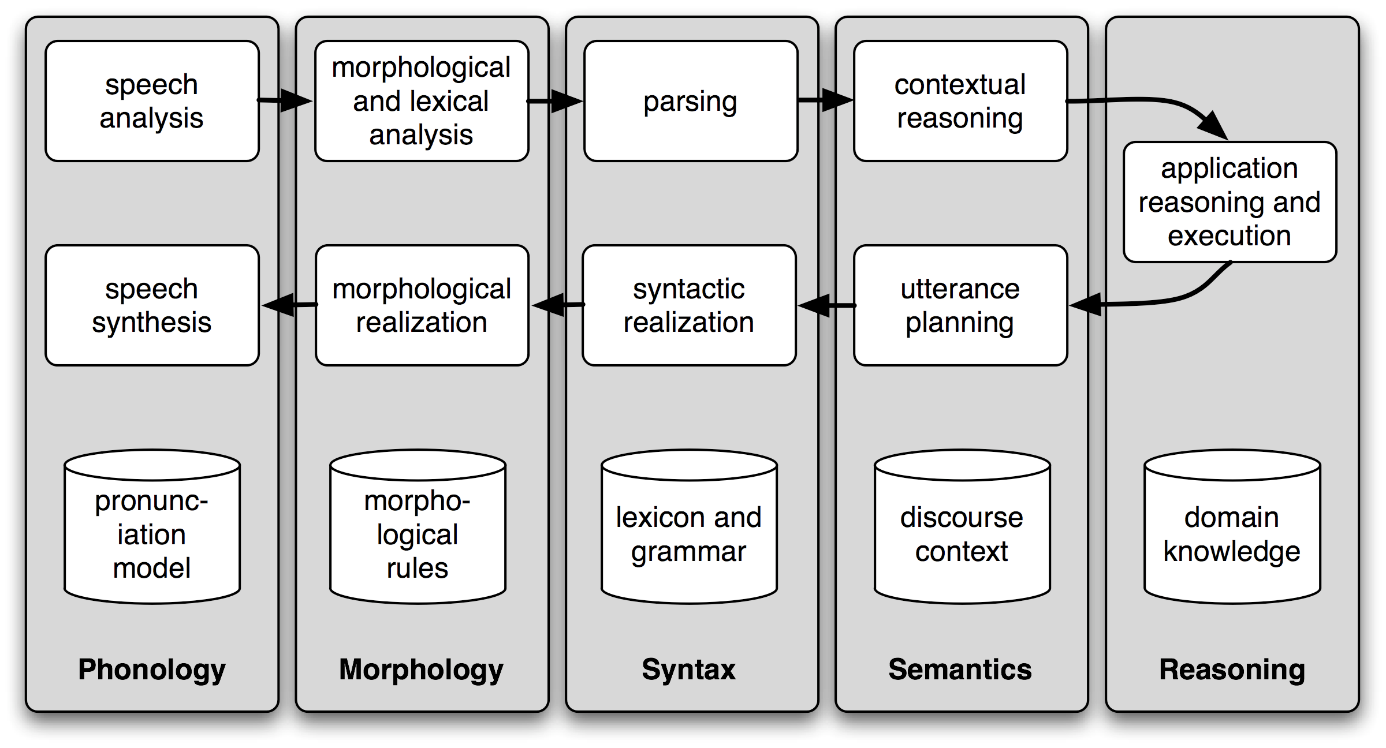
\includegraphics[width = \textwidth]{analyseDetaillee.png}
	\caption{Analyse NLP}
	\label{fig:Analyse NLP}
\end{figure}


\section{Dialogue chatbot}

On distingue principalement trois composants dans l’architecture d’un chatbot :
\vspace{1em}

\begin{itemize}
	\item L’interface utilisateur à travers laquelle les utilisateurs peuvent interagir avec le bot. 
	\item Un moteur qui traite les messages des utilisateurs et qui fonctionne avec une base de données pour stocker les données des utilisateurs et faire  appel à des services externes.
	\item Un moteur de Traitement Automatique du Langage Naturel qui transforme les entrées des utilisateurs en actions exécutables.
\end{itemize}
\vspace{1em}

Cette structure ressemble à  une architecture classique avec d’un côté un front-end et de l’autre un back-end qui expose une API. La grande différence est la présence du moteur du traitement du langage naturel.
\vspace{1em}

Voici l’architecture d’un chatbot :
\vspace{1em}

\begin{figure}[H]
	\centering
		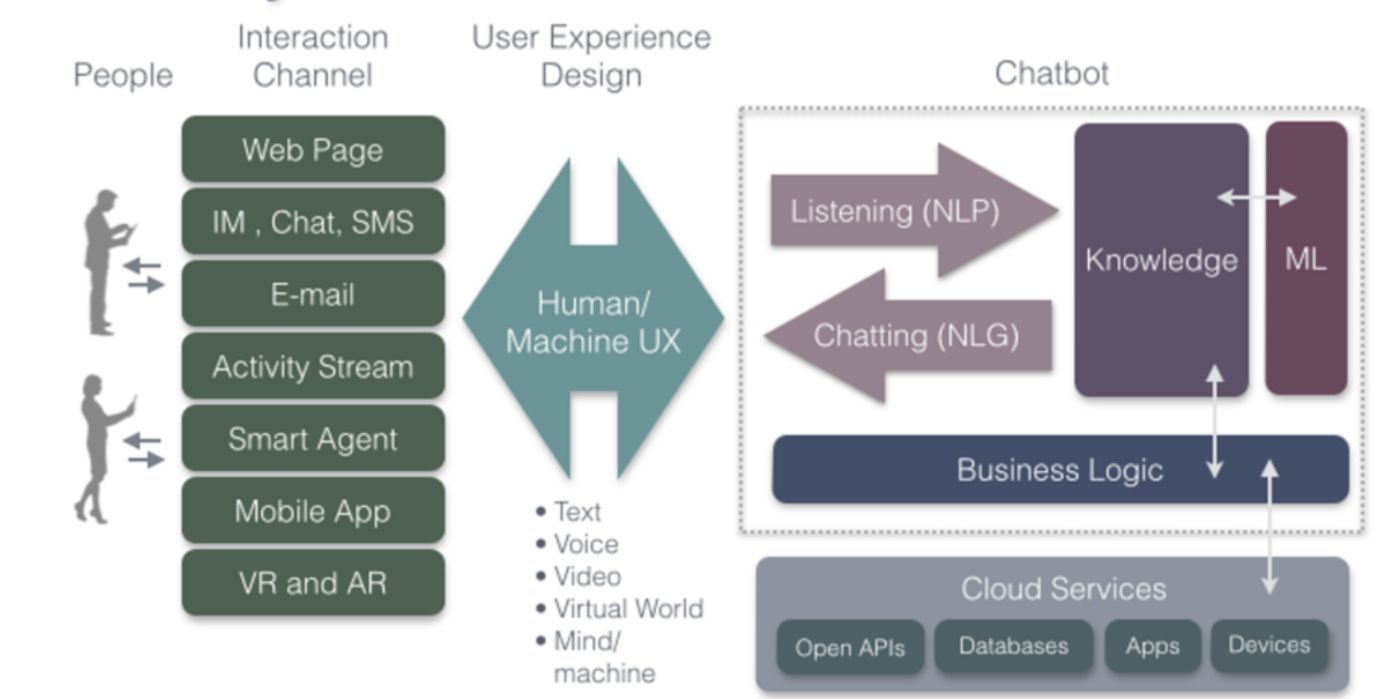
\includegraphics[width = \textwidth]{archiBot.png}
	\caption{Architecture d'un chatbot}
	\label{fig:Architecture d'un chatbot}
\end{figure}

On a la partie avec les différents canaux où les utilisateurs communiquent avec le chatbot sous différents formats tels que du texte, par la voix ou encore l’environnement.
\vspace{1em}

Dans le moteur de langue évoqué plus haut, on retrouve ici le NLP qui grâce aux connaissances et aux machine learning permettra au bot de comprendre le message de l’utilisateur. Ensuite il utilisera des règles en s’appuyant sur des services cloud pour formuler une réponse qui sera le NLG.